% headsectionstart
% update mixedReport hedsection if any changes done in this headsection
\documentclass{article}
\usepackage[a4paper, left=15pt, top=30pt, right=15pt, bottom=65pt]{geometry}
\usepackage{graphicx}
\usepackage{tikz}
\usepackage{atbegshi}
\usepackage{adjustbox}
\usepackage[sfdefault]{roboto}
\usepackage[colorlinks = true,
linkcolor = blue,
urlcolor  = blue,
citecolor = blue,
anchorcolor = blue]{hyperref}
\usepackage[printwatermark]{xwatermark}

\usetikzlibrary{fit,backgrounds,positioning,decorations.markings,shapes,arrows,shadows}
\definecolor{primary}{RGB}{115,54,163}
\definecolor{noVoteMessageBg}{HTML}{F9EADD}

\tikzset{
	headerText/.style={text=white},
	leftHeaderText/.style={headerText, align=left,text width=280pt},
	rightHeaderText/.style={headerText, align=right,text width=225pt},
	footerText/.style={text=white},
	leftFooterText/.style={footerText, align=left,text width=380pt},
	rightFooterText/.style={footerText, align=right,text width=193pt},
	noVotesMessageWidth/.style={text width=449pt}
}

\newcommand\Footer{%
  \sffamily
  \begin{tikzpicture}[remember picture,overlay]
  
    \node[leftFooterText] at (124pt, -734pt) (leftTop) {\Large Amount taken unethically from citizens in a rigged economy};
    \node[leftFooterText, below=-3pt of leftTop] (leftBottom) {Numbers and Theft vs. not Theft come from citizen voting
    and not ZTM Technologies SPC or this website};

    \node[rightFooterText, right=5pt of leftTop] (calculated) {--generatedTime-- \quad Page \thepage};
    \node[rightFooterText, below=0pt of calculated] (generatedBy) {Generated By \href{--holonUrl--}{\color{white}--holonUrl--}};

    \begin{scope}[on background layer]
    \node[fill=primary, fit=(leftTop)(leftBottom)(calculated)(generatedBy)] (footer) {};
    \end{scope}
  \end{tikzpicture}%
}

\pagestyle{empty}
\AtBeginShipout{\AtBeginShipoutAddToBox{\Footer}}

\newsavebox\mybox
\savebox\mybox{\tikz[color=gray,opacity=0.3]\node{Testing};}
\newwatermark*[
  pages=1-800,
  angle=45,
  scale=10,
  xpos=-20,
  ypos=15
]{\usebox\mybox}

\begin{document}
\sffamily
% headsectionend

\hypertarget{--pageID--}{}
% header
\trimbox{0 -15pt 0 0}{ 
  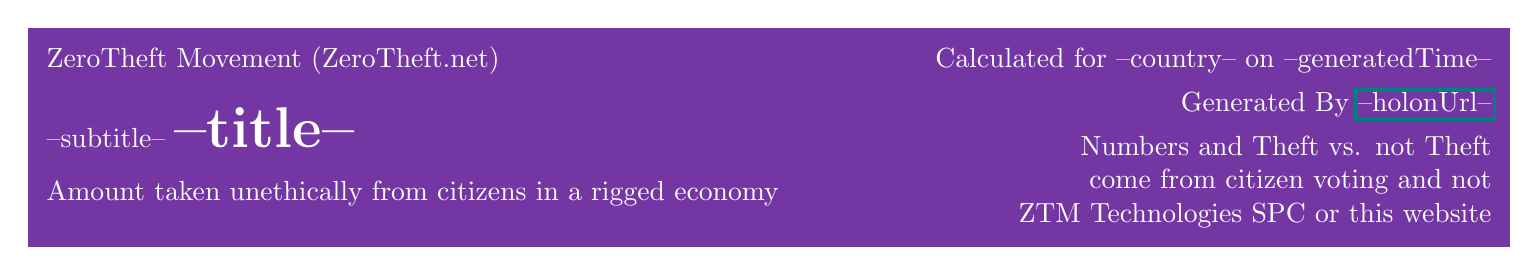
\begin{tikzpicture}
      \node[leftHeaderText] (top) {ZeroTheft Movement (ZeroTheft.net)};
      \node[leftHeaderText, below=5pt of top] (title) {--subtitle-- \huge \textbf{--title--}};
      \node[leftHeaderText, below=5pt of title] (belowtitle) {Amount taken unethically from citizens in a rigged economy};

      \node[rightHeaderText, right=10pt of top] (calculated) {Calculated for --country-- on --generatedTime--};
      \node[rightHeaderText, below=0pt of calculated] (generatedBy) {Generated By \href{--holonUrl--}{\color{white}--holonUrl--}};
      \node[rightHeaderText, below=0pt of generatedBy] (truth) {
        Numbers and Theft vs. not Theft come from citizen voting
        and not ZTM Technologies SPC or this website
      };
    
      \begin{scope}[on background layer]
      \node[fill=primary, fit=(top)(title)(belowtitle)(calculated)(generatedBy)(truth)] (header) {};
      \end{scope}
  \end{tikzpicture}
}

\trimbox{0 -15pt 0 0}{ 
  \begin{tikzpicture}
    \node(top){};
    \node[below=-20pt of top] (noVoteImage) {\includegraphics[width=60pt]{--pleaseVoteImage--}};
    \node[noVotesMessageWidth, align=center, below=10pt of noVoteImage] (title) {\Huge \textbf{Please Vote}};
    \node[noVotesMessageWidth, align=center, below=10pt of title] (message) {Looking for the voting results and the estimated amount of theft? As of now, no one has voted \\on this problem area. Be the first to weigh in on the matter, and make sure to get others \\involved as well!}; 
    \node[below=-20pt of message](bottom){};

    \begin{scope}[on background layer]
    \node[fill=noVoteMessageBg, fit=(top)(title)(message)(bottom), inner sep=40pt] (voteMessage) {};
    \end{scope}
  \end{tikzpicture}
}
\end{document}
